\chapter{Navegação}\label{cha:navigation}
Este capítulo descreve o mapa dinâmico e sua ajuda para a navegação, também descreve algumas informações de planeio e provas sobrepostas no mapa.

\section{Elementos mostrados no mapa}

\begin{maxipage}
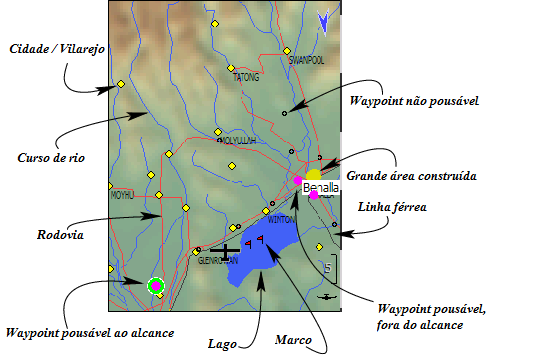
\includegraphics[angle=0,width=0.9\linewidth,keepaspectratio='true']{figures/fig-map.png}
\end{maxipage}

O mapa dinâmico mostra: 
\begin{enumerate} 
\item Aeronave, indicador de vento, perfil da termal, indicador de planeio final
\item Terreno, planícies e planaltos
\item Topografia, rios, rodovias e cidades
\item Waypoints, aeroportos e pousos
\item Prova ativa, zonas de observação e pilões
\item A direção (ou rota)\footnote {A linha até o próximo waypoint pode ser uma {\em route}, como descrição na seção~\ref{sec:route}.}) para a direção para o próximo waypoint.
\item Espaços aéreos
\item Marcadores, histórico de termais, trilha
\item Alcance do planeio\footnote{O alcance do planeio também é citado como
  {\em reach}, assim como descrito na seção ~\ref{sec:reach}.}
\end{enumerate}
O mapa é desenhado em um sistema de coordenadas projetadas (sem latitude e longitude), e a escala pode ser alterada (zoom + e zoom -), bem como deslocado.  Todas as funções de navegação levam a curvatura da Terra em consideração.

\section{Símbolo do planador, orientação do mapa}
O símbolo do planador mostra a posição da aeronave no mapa.  A orientação da aeronave indica a direção estimada que a aeronave está apontando.

O mapa é orientado de três formas: norte acima, trilha acima e alvo acima.  O ajuste da configuração pode ser utilizado para especificar uma orientação diferente no mapa quando estiver em modo de círculos.  É bem útil para prevenir a desorientação quando olhar o mapa girando.  O modo alvo acima facilita determinar em qual direção se deve sair da termal.

Quando o modo trilha ou alvo acima é usado no modo de círculos, o símbolo da aeronave é centralizado na tela, mesmo que o símbolo seja configurado de outra forma.  No modo de cruzeiro, a orientação de trilha e alvo acima permite que o símbolo da aeronave seja posicionado (ex. 20%) na parte inferior da tela, fornecendo uma boa visão do mapa a frente da aeronave.  Esta posição é definida nos ajustes da configuração.  

\section{Zoom e escala do mapa}\label{sec:zooming}

Para alterar a escala do mapa, dependendo do hardware, você usa:
\begin{enumerate}
\item 1.	Toque/clique em uma parte vazia do mapa para sublinhar o mapa se já não estiver selecionado.  Então utilize a roda do mouse ou as teclas acima/abaixo do Pocket PC para zoom + ou zoom -.
\item Um dispositivo PNA com um botão rotativo permite que se altere o zoom.
\item Dispositivos Android tem o +/- que permite que se altere o zoom.
\item Você pode também fazer o gesto para mudar o nível de zoom. Gesto acima (veja à esquerda) aumento o zoom.  Para baixo diminui o zoom.\gesturespec{up}
\item Ou selecione a função através do menu.
\begin{quote}
\bmenug{Display 1}\blink\bmenug{Zoom In} and \bmenug{Zoom Out}
\end{quote}
\item No Altair, o botão rotativo pode ser usado para alterar o zoom.
\end{enumerate}

A escala do mapa é mostrada no canto inferior do mapa dinâmico.  A distância indicada é medida da borda esquerda para a direita do mapa dinâmico.
Usuários do Compaq Aero.  Se você ativar as teclas de jogo do Compaq Aero (no Menu-Q), os dois botões centrais serão as teclas acima/abaixo.
\marginpar{\includegraphics[angle=0,width=0.4\linewidth,keepaspectratio='true']{figures/zoom.png}}

Usuários do Compaq Aero.  Se você ativar as teclas de jogo do Compaq Aero (no Menu-Q), os dois botões centrais serão as teclas acima/abaixo.

\subsection*{Zoom Girando}
THá uma facilidade de ter dois tipos de zoom: um quando a aeronave está em modo girando e outro em modo de cruzeiro ou modo final.  Esta é a opção de Zoom girando, nos ajustes das configurações.  Por padrão, o zoom girando é ajustado em 2,5 – 5,0km dependendo do tamanho da tela.  Quando o usuário altera o zoom, afeta diretamente o zoom atual somente.  Quando se sai do modo atual de zoom, é usado o modo prévio de zoom. Se o modo de Zoom girando não está ativo, haverá somente um único nível de zoom.  Esta situação conduz a diferentes níveis de zoom sendo preservados para serem alterados manualmente, independentemente dos ajustes de Auto Zoom.
 
\subsection*{Auto Zoom}
Auto Zoom automaticamente aproxima a tela quando se está aproximando de um waypoint 
para manter a visualização em uma distância apropriada.  
\marginpar{\includegraphics[angle=0,width=0.4\linewidth,keepaspectratio='true']{figures/zoomauto.png}}
Quando o Auto Zoom está ativo, ‘AUTO’ aparece perto da escala do mapa.

Para ativar o Auto Zoom, use o gesto \gesturespec{ud} ou o menu descrito à esquerda.  
Para voltar ao zoom normal, faça o zoom manualmente, não importando o que já foi 
feito por menu ou gesto. 

Quando um waypoint muda (automaticamente, através do seletor de prova ou manualmente 
\menulabel{\bmenug{Display 1}\blink\bmenut{Zoom}{Auto}}
selecionando waypoints), o Auto Zoom ajusta o nível de zoom automaticamente para que 
o próximo waypoint seja visível no mapa.

Durante o modo Girando se uma termal foi detectada, o mapa é centrado sobre a termal 
ou parte dela para que a aeronave continue sendo visível.
 
\section{Navegando no mapa (Panning)}\label{sec:panning}

O modo panorâmico permite ao usuário explorar áreas que estão além da aeronave.  É bem útil quando se está planejando a prova.
\begin{enumerate}
\menulabel{\bmenug{Display 1}\blink\bmenug{Pan On}}
\item E1.	Ative o modo panorâmico por menu ou gesto.  O gesto para este modo é mover sua ponta do dedo acima, direita, abaixo e esquerda, formando um “P”. 
\gesturespec{urdl}
\item O mapa pode ser movido arrastando a tela ou usando as teclas.  Para Altair, modo panorâmico é feito com o botão rotativo interno/externo.  
\item Quando feito, o modo panorâmico pode ser desabilitado manualmente, pressionando PAN OFF no sub-menu.
\end{enumerate} 

\sketch{figures/pan.png}
Quando o modo panorâmico está ativo, as letras ‘PAN’ aparecem próximas à escala do mapa.  Enquanto estiver nesse modo, o foco estará na mira no meio do mapa.

Apesar de aparecer a mira (para usuários Altair), o mapa continuará oferecendo a opção “Oque Aqui?” tocando em qualquer posição no mapa (na tela de toque). 


\section{Waypoints} \label{sec:waypoint-schemes}
Os waypoints são mostrados com símbolos diferentes, dependendo do tipo do waypoint; a maior diferença são waypoints pousáveis e não pousáveis.

\subsection*{Landables}
The waypoint symbols are drawn as shown below There are three icon sets for
landable waypoints. \config{waypointicons}

\begin{tabular}{c|ccc|ccc|}
Icon set 
&\begin{sideways}Pousável\end{sideways}
&\begin{sideways}Marginal\end{sideways}
&\begin{sideways}Alcançável\end{sideways}
&\begin{sideways}Aeródromo\end{sideways}
&\begin{sideways}Marginal\end{sideways}
&\begin{sideways}Alcançável\end{sideways}\\
\hline
Círculo Roxo &
\includegraphics[width=0.8cm]{icons/winpilot_landable.pdf} &
\includegraphics[width=0.8cm]{icons/winpilot_marginal.pdf} &
\includegraphics[width=0.8cm]{icons/winpilot_reachable.pdf} &
\colorbox{white}{\includegraphics[width=0.8cm]{icons/winpilot_landable.pdf}} &
\includegraphics[width=0.8cm]{icons/winpilot_marginal.pdf} &
\includegraphics[width=0.8cm]{icons/winpilot_reachable.pdf} \\
\hline
Branco e Preto &
\includegraphics[width=0.9cm]{icons/alt_landable_field.pdf} &
\includegraphics[width=0.9cm]{icons/alt_marginal_field.pdf} &
\includegraphics[width=0.9cm]{icons/alt_reachable_field.pdf} &
\colorbox[rgb]{0.94,0.94,0.94}{\includegraphics[width=0.9cm]{icons/alt_landable_airport.pdf}} &
\includegraphics[width=0.9cm]{icons/alt_marginal_airport.pdf} &
\includegraphics[width=0.9cm]{icons/alt_reachable_airport.pdf} \\
\hline
Luzes de tráfego &
\includegraphics[width=0.9cm]{icons/alt2_landable_field.pdf} &
\includegraphics[width=0.9cm]{icons/alt2_marginal_field.pdf} &
\includegraphics[width=0.9cm]{icons/alt_reachable_field.pdf} &
\colorbox{white}{\includegraphics[width=0.9cm]{icons/alt2_landable_airport.pdf}} &
\includegraphics[width=0.9cm]{icons/alt2_marginal_airport.pdf} &
\includegraphics[width=0.9cm]{icons/alt_reachable_airport.pdf} \\
\hline
\end{tabular} \\

Os ícones marginais são desenhados para aqueles waypoints que estão principalmente no alcance, mas não é possível a aproximação direta (ex. uma montanha não permite a aproximação direta).
  
Os waypoints são rotulados opcionalmente de acordo com suas abreviações, esquemas e visibilidade.

No topo dos waypoints pousáveis, pode haver mais detalhamento.  Se houver a opção ativada 
`{\it Detailed landables}' você terá informações adicionais quando houver a visualização deste waypoints.

\begin{enumerate}
\item  Campos pousáveis têm ícone quadrado apesar de serem mostrados em tabela.  O quadrado é desenhado como um diamante de pé em um canto.  Aeródromos permanecem com um círculo, facilitando sua visualização. 
\item  Todo o conjunto de ícones incluindo o conjunto de “círculos roxos”, colocam a pista em suas atuais direções.  A direção da pista está disponível nos dados do waypoints.  Ex. os waypoints de formato (\verb|.cup|) não incluem esta informação.
\end{enumerate}

\subsection*{Pousáveis ao Alcance}
Próximo aos pousáveis, há uma estimativa da altitude acima da altura de segurança dos 
pontos pousáveis e é mostrada próxima ao waypoints.  Esta característica é uma das 
capacidades mais poderosas do XCSoar.  A altitude de chegada é calculada configurando-se 
o computador de planeio do XCSoar com parâmetros de polar, ajustes de MacCready, vento, 
abertura do terreno e altitudes de segurança.  Com tudo isso sendo configurável, há muito 
espaço para erros, portanto:

A menos que tenha entendido completamente os conceitos de cálculo de planeio, você deve 
\warning manter a pré-configuração do XCSoar (já julgado e fortemente aprovada).

É da responsabilidade do piloto sempre interpretar a leitura e observar os valores com o 
tempo.  Todavia, tendo ajustado o computador de planeio seguindo o capítulo 
\ref{cha:glide} mostra a altitude estimada de alcance, desenhada ao lado de campos pousáveis ao alcance levam em consideração o relevo ou mostram ambos.

Outra opção é mostrar o planeio médio necessário para um campo pousável ao alcance.  Este cálculo é derivado da distância atual ao campo pousável dividido pela diferença de altura entre a altura atual e a altura do campo pousável.  Novamente, a altura de segurança é adicionada à altura do campo pousável, mas nada mais é levado em consideração: sem vento, sem polar, sem ajuste MacCready, só geometria.  O conceito do planeio médio necessário é amplamente discutido, como um conceito bem robusto.

\tip Tenha em mente que necessita de um forte conhecimento dos dados de alcance e ajustes no computador de planeio.

\subsection*{Não Pousáveis}
Como o arquivo de waypoints contém informações da natureza do campo não-pousável, o mapa mostrará ícones específicos para estes pontos.  A tabela contém uma relação dos ícones de mapas apresentados (veja figura  \ref{fig:nonlandables}).

\begin{figure}[h]
\centering
\vspace{2.5cm}
\begin{tabular}{ccccccccc}
\begin{rotate}{60}Waypoint simples\end{rotate} &
\begin{rotate}{60}Topo da montanha\end{rotate} &
\begin{rotate}{60}Obstáculo\end{rotate} &
\begin{rotate}{60}Passagem\end{rotate} &
\begin{rotate}{60}Planta ou fábrica\end{rotate} &
\begin{rotate}{60}Torre ou prédio\end{rotate} &
\begin{rotate}{60}Túnel\end{rotate} &
\begin{rotate}{60}Estação metereológica\end{rotate} &
\begin{rotate}{60}Ponte\end{rotate}\\

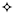
\includegraphics[width=0.5cm]{icons/map_turnpoint.pdf} &
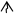
\includegraphics[width=0.8cm]{icons/map_mountain_top.pdf} &

\includegraphics[width=0.7cm]{icons/map_obstacle.pdf} &
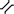
\includegraphics[width=0.7cm]{icons/map_pass.pdf} &
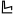
\includegraphics[width=0.8cm]{icons/map_power_plant.pdf} &
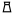
\includegraphics[width=0.7cm]{icons/map_tower.pdf} &
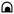
\includegraphics[width=0.6cm]{icons/map_tunnel.pdf} &
\includegraphics[width=0.6cm]{icons/map_weather_station.pdf} &
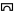
\includegraphics[width=0.8cm]{icons/map_bridge.pdf} \\

\end{tabular}
\caption{non-landables}\label{fig:nonlandables}
\end{figure}
\pagebreak

\section{Prova ativa}

O curso da prova ativa é desenhado no mapa em linha azul (pontilhada).  As áreas atribuídas às provas mostram os setores dos pilões ou áreas sombreadas em amarelo.  Círculos são desenhados ao redor dos pontos de início e fim, as linhas são desenhadas nos pontos de início e fim se os pontos são deste tipo.  Os setores de observação da prova são desenhados em segmentos de círculos.

A todo tempo, uma linha fina é desenhada da aeronave até o próximo waypoints da prova.  Esta linha deve ser um caminho direto ao waypoint, ou ser uma rota livre de terrenos e espaços aéreos, descritos anteriormente em detalhes na seção
~\ref{sec:route}.

\begin{center}
\begin{tabular}{c c c}
{\it Início/Fim} & {\it Setor} & {\it Cilindro} \\
\includegraphics[angle=0,width=0.3\linewidth,keepaspectratio='true']{figures/cut-startfinish.png} &
\includegraphics[angle=0,width=0.3\linewidth,keepaspectratio='true']{figures/cut-sector.png} &
\includegraphics[angle=0,width=0.3\linewidth,keepaspectratio='true']{figures/cut-barrel.png} \\
\end{tabular}
\end{center}


\section{Terreno e Topografia}\label{sec:terrain_topo}

As seguintes características de topografia são desenhadas no mapa:
\begin{itemize}
\item Rodovias principais, mostradas em linhas vermelhas
\item Rios, mostrados em linhas azuis
\item Grandes corpos de água (lagos), mostrados em áreas azuis
\item Cidades grandes, mostradas em áreas amarelas
\item SÁreas de pequena população, mostrada como diamantes amarelos 
\end{itemize}
Cidades e pequenas áreas com população são rotuladas em itálico.

O solo é colorido de acordo com a elevação e opcionalmente sombreado pelo sol ou pela direção do vento.  Solos inválidos ou abaixo do nível do mar são coloridos em azul.


\menulabel{\bmenug{Mostrar 2}\blink\bmenut{Terreno}{On/Off}}
\menulabel{\vspace{1cm}\bmenug{Display 2}\blink\bmenut{Topo.}{On/Off}}

O solo é sombreado para melhorar a visibilidade.  O sombreamento padrão é ajustado 
coincidindo a iluminação virtual com a direção do vento, sendo as áreas mais brilhantes 
são barlavento e as áreas mais escuras são sotavento.   
A inclinação solar também foi implementada.  Se o sombreamento da encosta for ajustado 
para ‘Sol’, o brilho da encosta segue conforme o dia e hora.  A quantidade de sombra sobre 
o brilho do terreno é ajustável \config{shading}.

A visualização do solo e topografia podem ser acionados ou não através do menu.

\begin{tabular}{c c}
Topography & Terrain \\
\includegraphics[angle=0,width=0.4\linewidth,keepaspectratio='true']{figures/cut-topo.png} &
\includegraphics[angle=0,width=0.4\linewidth,keepaspectratio='true']{figures/cut-terrain.png} \\
\end{tabular}

Se os dados do solo não estão disponíveis (ou a visualização está desligada), a cor de fundo do mapa será branca.  Todo o solo abaixo do nível médio do mar é mostrado em azul.  Se você estiver voando fora da terra, o fundo da tela será branco.  

\subsection*{Rótulos do mapa}\label{sec:maplabels}

A tela pode ser mais clara desligando a visualização dos rótulos de topografia e waypoints for a da prova escolhendo o menu ‘Rótulos’.
\menulabel{\bmenug{Mostrar 2}\blink\bmenut{Rótulos}{Nenhum}}

Outra opção para deixar mais clara incluem:

\jindent{\bmenuth{Rótulos}{Prova \&}{locais pouso}}{  Mostra rótulos para os waypoints na prova ativa e campos pousáveis (baseado nos atributos dos waypoints).  Os outros waypoints serão mostrados, mas sem rótulos. }

\jindent{\bmenut{Rótulos}{Prova}}{ Mostra somente os rótulos dos waypoints da prova ativa.}
\jindent{\bmenut{Rótulos}{Todos}}{ Mostra todos os rótulos para todos os waypoints.}

Note que em todos os casos, a formatação dos rótulos é configurável no menu
`{\it Waypoint Display}'.  \config{labels}


\section{Rastro}\label{sec:trail}


Um rastro opcional pode ser desenhado no mapa dinâmico para mostrar o caminho da aeronave.  A cor e a espessura do rastro dependem de altitude ou do valor do variômetro.


\begin{center}
\includegraphics[angle=0,width=0.5\linewidth,keepaspectratio='true']{figures/snail.pdf}
\end{center}

Se houver conexão do Vega ou outro variômetro inteligente com a saída Netto, o valor do vário Netto é usado; conseqüentemente as cores e a espessura do rastro indicarão o movimento vertical da massa de ar ao invés do movimento vertical da aeronave.

\config{snailtrail}
A visualização do rastro pode ser ajustada entre Desligado, Curto (+/- 10 minutos), Longo (+/- uma hora) ou Completo que mostrará todo o vôo.  Isto pode ser ajustado através dos ajustes de configuração ou temporariamente através do menu.
\menulabel{\bmenug{Mostrar 2}\blink\bmenut{Trilha}{Completo}}

Observe que para todos estes modos, o rastro é curto no modo Girando para facilitar a visualização.

De modo a auxiliar a centralização das térmicas na presença de vento, o rastro pode ser artificialmente derivado com o vento conforme vai sendo mostrado (é a compensação de deriva).  Deste modo, o rastro é referenciado pelo vento e não pelo solo.  Assim como as termais também são derivadas com o vento, o rastro pode dar uma indicação mais precisa onde esteve a aeronave com relação às termais.

O exemplo é ilustrado abaixo.  Observe que, quando há a compensação da deriva do vento está ativa, a aeronave aparenta estar girando em uma coluna ao invés de estar em uma espiral alongada (figura à esquerda).

\begin{center}
\includegraphics[angle=0,width=0.6\linewidth,keepaspectratio='true']{figures/traildrift.png}
\end{center}

\config{traildrift}
Ativando a compensação da deriva do rastro é através dos ajustes de no menu de configuração. A compensação só é feita no modo Girando; a visualização do rastro no modo Cruzeiro não é afetada.  Também pode ser alterada pela janela de ajuste do vento.
\menulabel{\bmenug{Config 1}\blink\bmenus{Vento}}

A visualização do rastro é útil também para mostrar mais claramente quando as termais são cisalhadas pela tesoura de vento.
A largura da trilha pode ser opcionalmente alterada de acordo com a visualização do variômetro.  


\section{Marcadores}\label{sec:markers}

Os marcadores são mostrados como pequenas bandeiras no mapa.  Os marcadores podem ser adicionados manualmente ou automaticamente.  Um exemplo de como estes marcadores podem ser adicionados automaticamente é quando se entra em modo Girando, um modo simples de mostrar as termais encontradas.

\menulabel{\bmenug{Nav 2}\blink\bmenut{Marca}{Ponto}}
Os marcadores não são mantidos após o XCSoar ser fechado, porém a localização dos marcadores é anexada ao arquivo \verb|xcsoar-marks.txt|.

\section{Termais}

Enquanto estiver girando em termais, automaticamente será gerado um marcado e mantido até o 
\sketch{figures/thermalhistory.png}
fim do vôo.  Este histórico termal é acessível através da função de elementos de mapa, da 
mesma forma que os marcadores ou waypoints.


\section{Linha de alcance de planeio}\label{sec:reach}

Uma linha de alcance de planeio é mostrada no mapa como uma linha pontilhada branca e 
preta, indicando onde a aeronave poderá pousar em terreno aberto.  O alcance é mostrado 
em todas as direções, incluindo caminhos obstruídos no terreno.  Esta opção é útil para 
conhecer o planeio relativo à topografia quando se está baixo e procura por termais, ou 
quando está voando em áreas montanhosas.

Os cálculos para o alcance podem ser configurados \config{turningreach} em dois níveis: 
\begin{description}
\item[Linha reta] se o alcance de curva está desabilitado, mostrará a maior distância 
que a aeronave pode voar no planeio final em todas as direções sem fazer curvas.  O 
alcance aparece como um anel fechado ao redor da aeronave.  

\begin{center}
\includegraphics[angle=0,width=0.8\linewidth,keepaspectratio='true']{figures/reach1.png}
% CUTOUT SHOWING GLIDE RANGE FOOTPRINT.  NO TOPOGRAPHY, FULLSCREEN, NO TASK. TURNING=FALSE
\end{center}

\item[Girando] se o modo Girando estiver ativo, o planeio será mostrado como a maior área 
que a aeronave pode alcançar em todas as direções, mesmo permitindo curvas ao redor de 
obstáculos3.  A área de alcance aparece com um anel fechado ao redor da aeronave mas 
também pode incluir buracos indicando picos de montanhas que a aeronave não pode alcançar 
sem subir.

\begin{center}
\includegraphics[angle=0,width=0.8\linewidth,keepaspectratio='true']{figures/reach2.png}
% CUTOUT SHOWING GLIDE RANGE FOOTPRINT.  NO TOPOGRAPHY, FULLSCREEN, NO TASK. TURNING=TRUE
\end{center}

\end{description}

A tela pode ser configurada também para desfocar as áreas não alcançáveis fora do alcance do planeio da aeronave.  O caminho do planeio final é verificado levando-se em consideração também a abertura do terreno através do caminho e também a altura do terreno.
Se a abertura (clareza) do terreno não é alcançada, aparecerá uma cruz vermelha no mapa onde a área é perigosa.  Se um alvo for definido, os cálculos são feitos através do caminho reto para o alvo.  Se não há alvo definido, o cálculo é feito através do caminho que está seguindo.
Se o alcance estiver ativo, então o modo de aborto de prova usará os waypoints pousáveis e abrirá uma lista também com os waypoints alternativos do mapa.
Observe que os cálculos da prova não são afetados pelos cálculos de alcance – por exemplo, não são levando em conta os dados de altitude necessária para finalizar a prova e dados mostrados nas infoboxes.

Além do mais, os cálculos são usados para o anel de alcance, altura de chegada para waypoints pousáveis, modo de aborto e janelas de diálogo alternativas.  O desempenho da aeronave e os ajustes de MacCready usados nestes cálculos são configuráveis\config{reachpolar}:
\begin{description}
\item[Prova] O valor de MC é o usado na prova.
\item[Safety MC] Um valor de MC baixo pode ser configurado para ser usado como referencial ao melhor planeio da aeronave.  O grau de segurança alcançado nos cálculos é feito com a diferença entre o melhor desempenho de planeio e o planeio seguindo o Safety MC (speed to fly).  
\end{description}

\section{Abas de estado `{\it Voo}' and `{\it Tempo}'}\label{sec:flight-status}

A janela de diálogo Estado é multi-tabular, fornecendo uma visão geral da informação do vôo, sistema, prova, regras e tempos.  Pode ser acessada com o gesto “S” ou com o botão do Menu. 
\gesture{Esquerda - Baixo - Direita - Baixo - Esquerda}
\begin{quote}
\bmenug{Info 2}\blink\bmenug{Estado}
\end{quote}

\subsection*{Vôo}
Selecione a página `{\it Flight}'. 
A janela mostra a localização da aeronave e pode ser útil quando se reporta a posição.  Mostra a posição da aeronave, o máximo ganho de altura, waypoints mais próximo, ângulo de direção e distância.
\sketch{figures/status-flight.png}

Você pode achar esta função útil quando for reportar sua localização para outros pilotos ou resgate.

\subsection*{Tempo}\label{sec:time-status}
Seleciona a aba  `{\it Times}'. 
Mostrará a hora local, tempo de vôo, hora da decolagem e pouso e hora do nascer e pôr do sol.

Observe que estes valores nesta aba são estáticos e só serão atualizados a cada abertura de aba. 
\sketch{figures/status-times.png}
Para ver os dados atualizados, é necessário fechar a aba e abrí-la novamente.  Os valores serão atualizados. 


\section{Rota}\label{sec:route}

O XCSoar pode planejar caminhos pelo terreno e obstáculos no espaço aéreo em três dimensões da aeronave até o destino.  Este caminho é conhecido como rota.  A altura do destino é a altura de chegada para waypoints finais ou pode ser mais alto para waypoints intermediários, se forem regras da prova ou requisitos para completar a prova.  

As funções de planejamento de rota são ordenadas por modo de prova, modo de aborto e modo ‘ir para’.

\begin{center}
\includegraphics[angle=0,width=0.8\linewidth,keepaspectratio='true']{figures/route3.png}
\end{center}

As rotas levam em consideração o desempenho da polar e são calculadas para levarem o mínimo 
tempo.  Por padrão, os cálculos de rota são desativados e podem ser ativados somente por 
solo ou, prevenção de espaço aéreo. \config{routemode}.

O solo é evitado verticalmente pela altura de segurança do terreno
\config{safetyterrain}, sem nenhuma abertura de terreno lateral.  As rotas válidas podem 
resultar na chegada da aeronave ao destino mais alta que a altura mínima – como pode 
ocorrer quando o destino está além de uma montanha mais alta.

O espaço aéreo é evitado horizontalmente por uma margem de aproximadamente 250m sem 
nenhuma abertura imposta verticalmente.  As rotas válidas podem voar acima ou abaixo 
do espaço aéreo.

Se o MacCready é positivo, a subida é opcionalmente permitida nos cálculos de rota.  O 
topo da subida deve ser limitado a 500m acima do teto de início e final, ou incluso no 
teto, definido pelo teto da termal %\config{routeceiling}.  
As subidas acima da altitude 
de início e final são penalizadas por uma taxa de subida mais lenta que o valor de 
MacCready atual.

Algumas aproximações e limitações do sistema de planejamento de rotas são:
\begin{itemize}
\item Quando subidas são necessárias (e permitidas) para alcançar o destino, as subidas podem ocorrer no início da rota. 
\item Segmentos de subidas em cruzeiro podem ocorrer em altitude constante, equivalente a muitas pequenas subidas distribuídas ao longo do caminho. 
\item Falhas sobre o resultado dos cálculos podem se reverter em vôo direto da aeronave, de sua localização atual para o destino.
\end{itemize}

